\documentclass[14pt]{article}
\title{Lab2 Report}
\author{Zepeng Chen}
\date{\today}
\usepackage{listings}
\usepackage{color}
\usepackage{graphicx}
\usepackage{subcaption}
\usepackage{gensymb}
\usepackage{geometry}
\geometry{a4paper,left=2cm,right=2cm,top=1cm,bottom=1cm}

\definecolor{dkgreen}{rgb}{0,0.6,0}
\definecolor{gray}{rgb}{0.5,0.5,0.5}
\definecolor{mauve}{rgb}{0.58,0,0.82}

\lstset{frame=tb,
	language=Python,
	aboveskip=3mm,
	belowskip=3mm,
	showstringspaces=false,
	columns=flexible,
	basicstyle={\small\ttfamily},
	numbers=none,
	numberstyle=\tiny\color{gray},
	keywordstyle=\color{blue},
	commentstyle=\color{dkgreen},
	stringstyle=\color{mauve},
	breaklines=true,
	breakatwhitespace=true,
	tabsize=3
}

\begin{document}
	\maketitle
	\tableofcontents
	\section{Spatial Filtering}
	\subsection{Integrated Function including linear and nonlinear filter}
	\lstinputlisting[breaklines]{lab2.py}
	\newcommand{\RNum}[1]{\uppercase\expandafter{\romannumeral #1\relax}}
	\subsection{Outcome Collections \RNum{1}}

	\begin{figure}[hbt!]
		\centering
		\begin{subfigure}[b]{0.23\linewidth}
			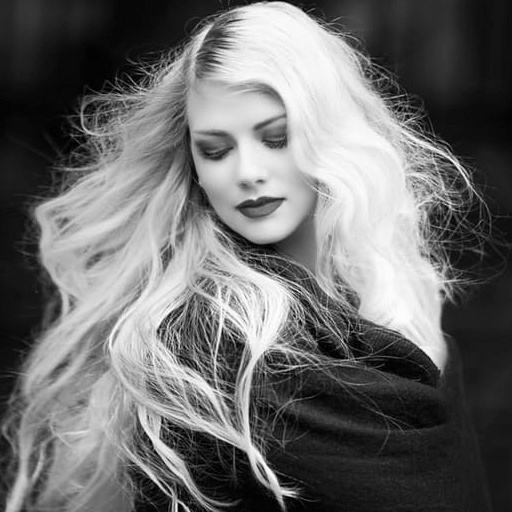
\includegraphics[width=\linewidth]{origin1.png}
			\caption{Img1 Original Image.}
		\end{subfigure}
		\begin{subfigure}[b]{0.23\linewidth}
			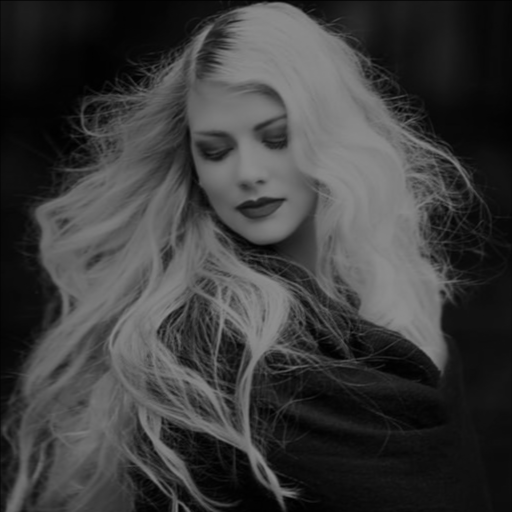
\includegraphics[width=\linewidth]{ones3.png}
			\caption{Ones(3)}
		\end{subfigure}
		\begin{subfigure}[b]{0.23\linewidth}
			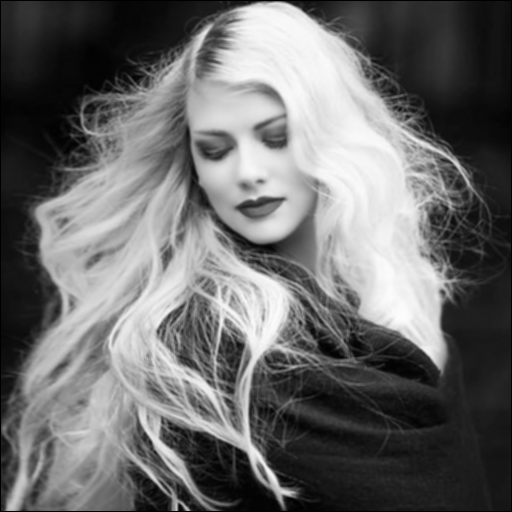
\includegraphics[width=\linewidth]{ones7.png}
			\caption{ones(7)}
		\end{subfigure}
		\begin{subfigure}[b]{0.23\linewidth}
			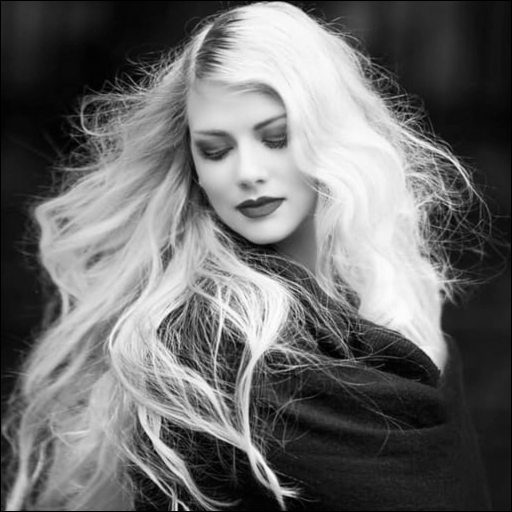
\includegraphics[width=\linewidth]{g3.png}
			\caption{Gaussian3}
		\end{subfigure}
		\begin{subfigure}[b]{0.23\linewidth}
			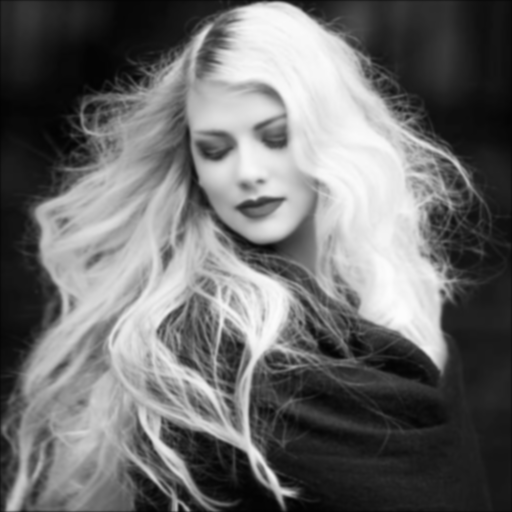
\includegraphics[width=\linewidth]{g7.png}
			\caption{Gaussian7}
		\end{subfigure}
		\begin{subfigure}[b]{0.23\linewidth}
			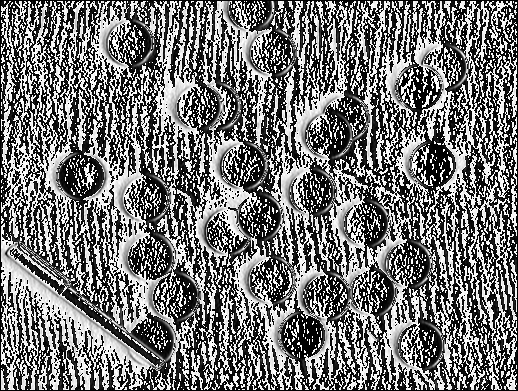
\includegraphics[width=\linewidth]{k6.png}
			\caption{Sobel-x}
		\end{subfigure}
		\begin{subfigure}[b]{0.23\linewidth}
			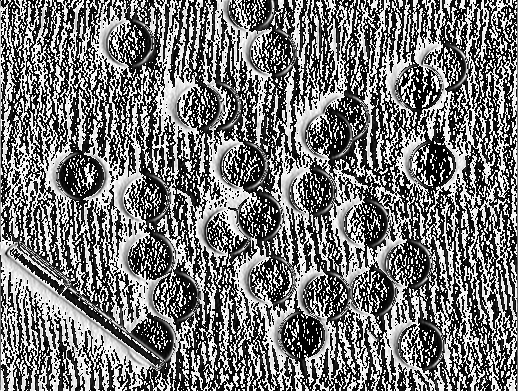
\includegraphics[width=\linewidth]{k7.png}
			\caption{Sobel-y}
		\end{subfigure}
		\begin{subfigure}[b]{0.23\linewidth}
			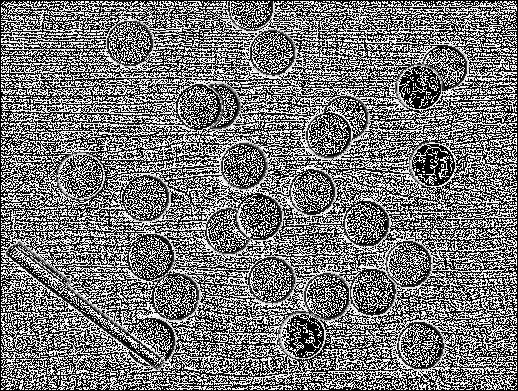
\includegraphics[width=\linewidth]{k8.png}
			\caption{log3}
		\end{subfigure}
	\end{figure}

	\subsection{Median Filter Outcome}

	\begin{figure}[hbt!]
		\centering
	\begin{subfigure}[b]{0.3\linewidth}
		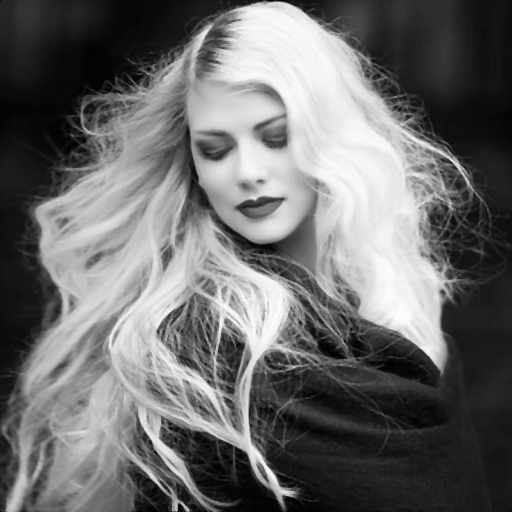
\includegraphics[width=\linewidth]{m3.png}
		\caption{Median3X3}
	\end{subfigure}
	\begin{subfigure}[b]{0.3\linewidth}
		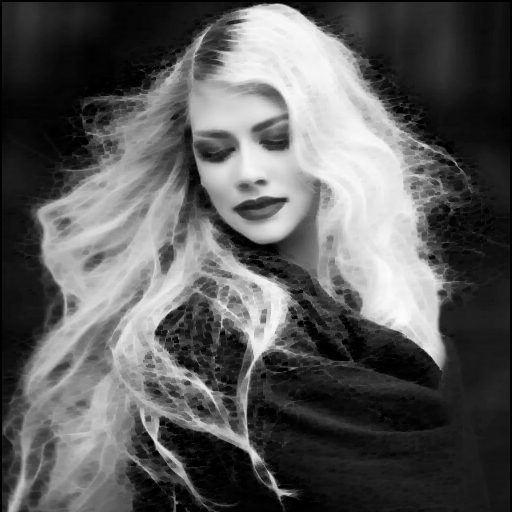
\includegraphics[width=\linewidth]{m5.png}
		\caption{Median5X5}
	\end{subfigure}
	\end{figure}
\newpage
\section{Thresholding}
\subsection{Code for fingding threshold}
\lstinputlisting[breaklines]{thresholding.py}
\subsection{Outcome}

\begin{figure}[hbt!]
	\centering
	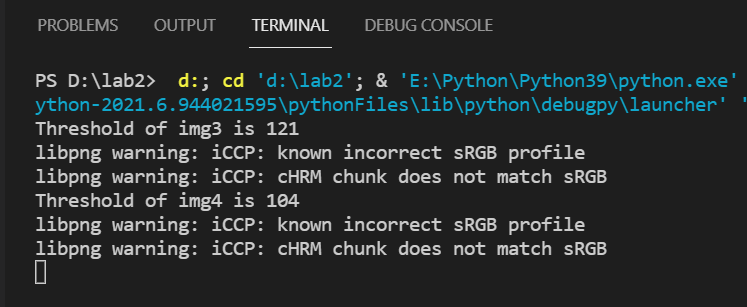
\includegraphics[width=\linewidth]{thValue.png}
	\caption{Threshold of img3 and img4 executed from function.}	
\end{figure}
\begin{figure}[hbt!]
	\centering
	\begin{subfigure}[b]{0.4\linewidth}
		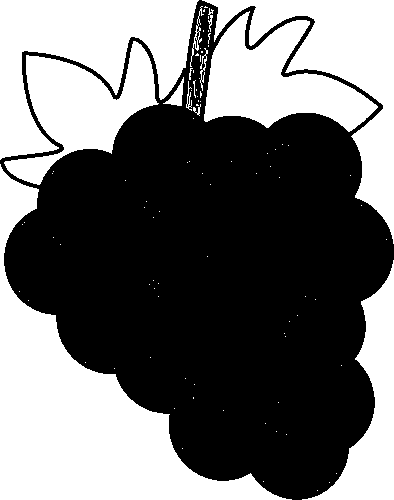
\includegraphics[width=\linewidth]{img3bi.png}
		\caption{Binarized img3}
	\end{subfigure}
	\begin{subfigure}[b]{0.4\linewidth}
		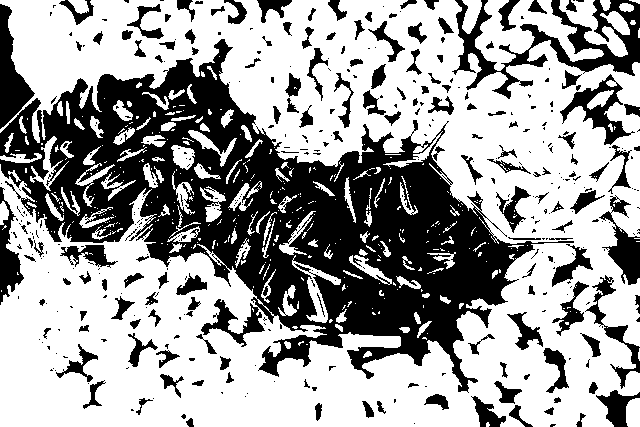
\includegraphics[width=\linewidth]{img4bi.png}
		\caption{Binarized img4}
	\end{subfigure}
\end{figure}
\section{Discussion}
1.Kernel1 and kerne5 are avaraging filter and gaussian filter. Compared to averaging filter, guassian filter weighs the pixel within the kernel which give higher weight to the closer pixel. So Gaussian highlight more importance for the colse pixel.\\
2. The bigger the kernel size is, the vaguer the image is. Becasue with a bigger size kernel, more pixels far from the origin which are less relevant to the origin pixel will be convolved.\\
3.Kernel6 is sobel filter for x axis, which sharpens the x direction edge. Kernel7 is a rotationally symmetric Laplacian of Gaussian filter, which sharpens the edge without direction feature.\\
4. Edges in an image represents a swift change in the intensity of an image and noise in an image also signifies the same. so when noise is abundant in an image, it can interfere the edge detection.\\
5.Adaptive thresholding typically takes a grayscale or color image as input and, in the simplest implementation, outputs a binary image representing the segmentation. For each pixel in the image, a threshold has to be calculated. If the pixel value is below the threshold it is set to the background value, otherwise it assumes the foreground value.
\end{document}